\graphicspath{{6setsii/asy/}}

\section{Set Theory, Part II}\label{chap:sets2}

In this chapter we return to set theory and consider several more-advanced constructions.


\subsection{Cartesian Products}\label{sec:cartprod}

You have been working with Cartesian products for years, referring to a point in the plane $\R^2$ by its \emph{Cartesian co-ordinates} $(x,y)$, an \emph{ordered pair} where each co-ordinate ($x,y$) is a member of the set $\R$. The same approach can be used for any sets.

\begin{defn}{}{}
	The \emph{Cartesian product} of sets $A$ and $B$ is the set of ordered pairs
	\[
		A\times B=\bigl\{(a,b):a\in A\text{ and }b\in B\bigr\}
	\]
	Otherwise said: $(a,b)\in A\times B\iff a\in A$ and $b\in B$.
\end{defn}

\begin{examples}{}{}
	\exstart The Cartesian product of the real line $\R$ with itself is the usual $xy$-plane.
	\begin{enumerate}\setcounter{enumi}{1}
	\begin{minipage}[t]{0.7\linewidth}\vspace{-8pt}
		\item[]As you've seen in other classes, rather than writing $\R\times\R$ which is unwieldy, we denote this set
		\[
			\R^2=\bigl\{(x,y):x,y\in\R\bigr\}
		\]
		More generally, the set of $n$-tuples of real numbers is\footnotemark
		\[
			\R^n=\bigl\{(x_1,x_2,\ldots,x_n):x_1,x_2,\ldots,x_n\in\R\bigr\} =\underbrace{\R\times\R\times\cdots\times\R}_{\text{$n$ times}}
		\]
	\end{minipage}
	\hfill
	\begin{minipage}[t]{0.29\linewidth}\vspace{-8pt}
		\flushright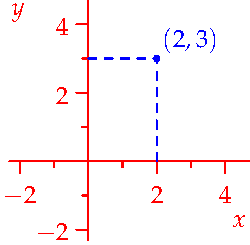
\includegraphics{setsii-cartesianplane}
	\end{minipage}

		\item If $A=\{1,2,3\}$ and $B=\{\alpha,\beta\}$, then the Cartesian product of $A$ and $B$ is
		\[
			A\times B=\bigl\{(1,\alpha),\ (1,\beta),\ (2,\alpha),\ (2,\beta),\ (3,\alpha),\ (3,\beta)\bigr\}
		\]
		The order of terms in an ordered pair really matters: the Cartesian product with the roles reversed is 
		\[
			B\times A=\bigl\{(\alpha,1),\ (\beta,1),\ (\alpha,2),\ (\beta,2),\ (\alpha,3),\ (\beta,3)\bigr\}
		\]
		While $A\times B\neq B\times A$, note that both Cartesian products have \emph{six} $(=3\cdot 2=2\cdot 3)$ elements.
		
		\item The menu in a restaurant might be summarized set-theoretically:
		\begin{gather*}
			\text{Mains}=\{\text{fish, steak, eggplant, pasta}\}, \qquad \text{Sides}=\{\text{asparagus, salad, potatoes}\}
		\end{gather*}
		The Cartesian product Mains\,$\times$\,Sides is the set of all possible meals consisting of one main and one side. It should be obvious that there are $4\times 3=12$ possible meal choices.
	\end{enumerate}
\end{examples}

\footnotetext{Strictly this should be defined inductively, e.g., $\R^3:=\R^2\times\R=\Bigl\{\bigl((x,y),z\bigr):x,y,z\in\R\Bigr\}$, but this is very tedious!}

The last two examples illustrate one of the simplest properties of Cartesian products, in a result which indeed justifies the very use of the word \emph{product}!

\begin{thm}{}{}
	If $A$ and $B$ are finite sets, then $\nm{A\times B}=\nm A\cdot\nm B$.
\end{thm}

\begin{proof}
	Label the elements of each set and list the elements of $A\times B$ lexicographically. If $\nm A=m$ and $\nm B=n$, then
	\[
		\begin{array}{rccccccl}
			A\times B=\big\{&(a_1,b_1),&(a_1,b_2),&(a_1,b_3),&\cdots&(a_1,b_n),&\\
			&(a_2,b_1),&(a_2,b_2),&(a_2,b_3),&\cdots&(a_2,b_n),&\\
			&\vdots&\vdots&\vdots&&\vdots&\\
			&(a_m,b_1),&(a_m,b_2),&(a_m,b_3),&\cdots&(a_m,b_n)&\big\}
		\end{array}
	\]
	Every element of $A\times B$ is listed exactly once. There are $m$ rows and $n$ columns, so $\nm{A\times B}=mn$.
\end{proof}

\boldinline{Set Identities}

These may be established as we've done previously (Section \ref{chap:sets}): convert everything into propositions regarding elements of sets and use basic logic. If you're feeling more confident, you might also be able to invoke previously established rules of set algebra.

\begin{examples}{}{cartex}
	 	\exstart Consider the complement of a Cartesian product $A\times B$. If you had to guess an expression for $\comp{(A\times B)}$, you might mistakenly think it is $\comp A\times\comp B$. Let us think more carefully:
		\begin{align*}
			(x,y)\in\comp{(A\times B)}&\iff \neg((x,y)\in A\times B) \tag{definition of complement}\\
			&\iff \neg(x\in A\text{ and }y\in B) \tag{definition of $A\times B$}\\
			&\iff x\not\in A\text{ or }y\not\in B \tag{de Morgan (logic)}
		\end{align*}
		By contrast, $(x,y)\in\comp A\times\comp B\iff x\notin A\text{ and }x\notin B$, so $\comp{(A\times B)}\neq \comp A\times\comp B$. Indeed the complement of a Cartesian product is \emph{not a Cartesian product!} For more on this, see Exercise \ref{ex:cartneg}.

	\begin{enumerate}\setcounter{enumi}{1}
		\item\label{ex:cartex2}	Let $A,B,C,D$ be any sets. We prove that $(A\times B)\cup(C\times D)\subseteq(A\cup C)\times(B\cup D)$.
		\begin{align*}
			(x,y)\in(A\times B)\cup(C\times D)&\implies (x,y)\in A\times B \text{ or }(x,y)\in C\times D\\
			&\implies (x\in A\text{ and }y\in B)\text{ or }(x\in C\text{ and }y\in D)\\
			&\mathrel{\textcolor{red}{\implies}} (x\in A\text{ or }x\in C)\text{ and }(y\in B\text{ or }y\in D)\\
			&\implies x\in A\cup C\text{ and }y\in B\cup D\\
			&\implies (x,y)\in (A\cup C)\times(B\cup D)
		\end{align*}
		\begin{minipage}[t]{0.66\linewidth}\vspace{0pt}
			All implications except the \textcolor{red}{red arrow} are in fact \emph{biconditional.} To convince yourself of its truth, first consider what must be true about $x$, then do the same for $y$. The picture provides a visualization where $A,B,C,D$ are intervals of real numbers:
			\begin{itemize}\itemsep2pt
			  \item $(A\times B)\cup(C\times D)$ is the solid shaded region.
			  \item $(A\cup C)\times(B\cup D)$ is the larger dashed square.
			\end{itemize}  If $x\in C\setminus A$ and $y\in B\setminus D$, then $(x,y)\in (A\cup C)\times (B\cup D)$ but $(x,y)\not\in (A\times B)\cup(C\times D)$, so we do not, in general, expect these sets to be equal.
		\end{minipage}
		\hfill
		\begin{minipage}[t]{0.32\linewidth}\vspace{0pt}
			\hfill
			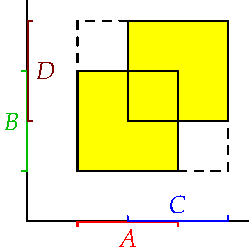
\includegraphics{setsii-04-cartesian}
		\end{minipage}
	\end{enumerate}
\end{examples} 



\begin{exercises}{}{}
	A reading quiz and several questions with linked video solutions can be found \href{http://www.math.uci.edu/~ndonalds/math13/selftest/6-1-cartprod.html}{online}.

	\begin{enumerate}
	  \item\begin{enumerate}
	    \item Suppose that $A=\{1,2\}$ and $B=\{3,4,5\}$. State the set $A\times B$ in roster notation.
	    \item Sketch both $A\times B$ and $B\times A$ using dots in $\R^2$. What do you observe about your pictures?
	    \item If $A,B,C$ are any sets, we may define
	    \[
	    	A\times B\times C=\bigl\{(a,b,c):a\in A,\ b\in B,\ c\in C\bigr\}
	    \]
	    If $C=\{6,7\}$ and $A,B$ are as above, state the set $A\times B\times C$ in roster notation.
	  \end{enumerate}
	
	
		\item Rewrite the condition $(x,y)\in (\comp{A}\cup B)\times (C\setminus D)$ in terms of (some of) the propositions
		\[
			x\in A,\quad x\not\in A,\quad x\in B,\quad x\not\in B,\quad y\in C,\quad y\not\in C,\quad y\in D,\quad y\not\in D
		\]
	  
	  
	  \item Consider the intervals $A=[2,5]$ and $B=(0,4)$ of real numbers.
	  \begin{enumerate}
	    \item Express the set $\comp{(A\setminus B)}$ in interval notation, as a disjoint union of intervals.
	    \item Draw a picture of the set $\comp{(A\setminus B)}\times (B\setminus A)$.
	  \end{enumerate}
	  (\emph{Be careful: In this problem $B=(0,4)$ is an \textbf{interval} (a subset of $\R$), not a \textbf{point} in $\R^2$!})
	
		
		\item A \emph{straight line} in $\R^2$ is a subset of the form
		\[
			A_{a,b,c}=\bigl\{(x,y):ax+by=c\bigr\},\quad\text{for some constants $a,b,c$, with $a,b$ not both zero}
		\]
		\begin{enumerate}
		  \item Draw the set $A_{1,2,3}$. Is it a Cartesian product?
		 	\item Which straight line subsets in the plane $\R^2$ are Cartesian products? Otherwise said, find a condition on the constants $a,b,c$ for which the set $A_{a,b,c}$ is a Cartesian product.
		\end{enumerate}
		
		
		\item\label{ex:cartneg} Draw a picture, similar to that in Example \ref*{ex:cartex}.\ref{ex:cartex2}, which illustrates the fact that
		\[
			\comp{(A\times B)} =(\comp A\times\comp B)\cup (\comp A\times B) \cup (A\times\comp B)
		\]
		Now give a rigorous proof of the claim.
		
		
		\item Let $A=[1,3]$, $B=[2,4]$ and $C=[2,3]$. Prove or disprove:
		\[
			(A\times B)\cap (B\times A)=C\times C
		\]
		(\emph{Hint: Draw the sets $A\times B$, $B\times A$ and $C\times C$ in the Cartesian plane})
		
			
		\item Prove that $A\cap B=\emptyset\iff (A\times B)\cap(B\times A)=\emptyset$.\par
		(\emph{Hint: try the previous question first})
		
		
		\item Let $A,B,C$ be sets. Prove:
		\begin{enumerate}
	  	\item $A\times (B\cup C)=(A\times B)\cup (A\times C)$
	    \item $A\times (B\cap C)=(A\times B)\cap (A\times C)$
	    \item $A\times (B\setminus C)=(A\times B)\setminus (A\times C)$
		\end{enumerate}
	
	
		\item\begin{enumerate}
	    \item Give an explicit example of sets $A,B,C,D$ such that
	    \[
	    	(A\times B)\cup (C\times D)\neq (A\cup C) \times (B\cup D)
	    \]
	    \item For any sets $A,B,C,D$, prove that
	    \[
	      (A\cup C)\times (B\cup D)=(A\times B)\cup (A\times D)\cup (C\times B)\cup (C\times D)
	    \]
		\end{enumerate}
		
		
	  \item Prove by induction. For all $n\in\N$, if $A_1,\ldots,A_n$ are finite sets, then
	  \[
	  	\nm{A_1\times\cdots\times A_n}=\nm{A_1}\cdots\nm{A_n}
	  \] 
	
		
	  \item\begin{enumerate}
			\item Suppose $\nm A=3$, and $\nm B=4$. What are the minimum and maximum values for the cardinalities $\nm{(A\times B)\cap(B\times A)}$ and $\nm{(A\times B)\cup(B\times A)}$?
			\item (Hard)\lstsp More generally, suppose $\nm A=m$, $\nm B=n$ and $\nm{A\cap B}=c$. What can you say about the cardinalities $\nm{(A\times B)\cap(B\times A)}$ and $\nm{(A\times B)\cup(B\times A)}$?
		\end{enumerate}
		
	
		\item Let $A$ and $B$ be nonempty sets. Define functions $\pi_1:A\times B\to A$ and $\pi_2:A\times B\to B$ by $\pi_1(a,b)=a$ and $\pi_2(a,b)=b$ respectively (these are called \emph{projection maps}). 
		\begin{enumerate}
	    \item If $A=B=\R$ and $X=[1,3]$, $Y=(2,4]$, then $X\times Y\subseteq A\times B$. Compute the images $\pi_1(X\times Y)$ and $\pi_2(X\times Y)$.
	    \item Let $Z$ be any set and suppose there are functions $\rho_1:Z\to A$ and $\rho_2:Z\to B$. Show that there is a unique function $h:Z\to A\times B$ such that $\rho_1=\pi_1\circ h$ and $\rho_2=\pi_2\circ h$.
		\end{enumerate}
		
		
		\item Let $E\subseteq\N\times\N$ be the smallest subset satisfying the following conditions:
		\begin{itemize}
			\item Base case: $(1,1)\in E$
			\item Generating Rule I: If $(a,b)\in E$ then $(a,a+b)\in E$
			\item Generating Rule II: If $(a,b)\in E$ then $(b,a)\in E$
		\end{itemize}
		\begin{enumerate}
			\item Show in detail that $(4,3)\in E$.
			\item Show by induction that for every $n\in\N$, $(1,n)\in E$.
			\item (Hard!)\lstsp Show that $E=\bigl\{(a,b)\in\N\times\N:\gcd(a,b)=1\bigr\}$.\par
			(\emph{Hint: what do the generating rules have to do with the Euclidean algorithm?})
		\end{enumerate}
		
		\item\label{exs:ordpairdef} (Hard)\lstsp A strict set-theoretic definition requires that ordered pair $(a,b)$ be defined as a set for instance $(a,b):=\bigl\{a,\{a,b\}\bigr\}$. We \emph{prove} that $(a,b)=(c,d)\Longleftrightarrow a=c$ and $b=d$.
		\begin{enumerate}
		  \item The \emph{regularity axiom} of set theory says there is no set $a$ for which $a\in a$. Use this to prove that the cardinality of $\bigl\{a,\{a,b\}\bigr\}$ is two.
		  \item Prove that $(a,b)=(c,d)\implies \bigl(a=c\text{ and }b=d\bigr) \text{ or }\bigl(a=\{c,d\}\text{ and }c=\{a,b\}\bigr)$
		  \item In the second case, prove that there exists a set $S$ such that $a\in S\in a$. The axiom of regularity also says that this is illegal. Conclude that $(a,b)=(c,d)\iff a=c$ and $b=d$.
		\end{enumerate}
		
	\end{enumerate}

\end{exercises}


\clearpage


\subsection{Power Sets}\label{sec:power}

Thus far we have used the operations of subset, complement, union, intersection and Cartesian product to build new sets from old. There is essentially only one further method available.

\begin{defn}{}{}
	Let $A$ be a set. Its \emph{power set} $\cP(A)$ is the set of all subsets of $A$:
	\[
		\cP(A)=\bigl\{B:B\subseteq A\bigr\}
	\]
	Otherwise said: $B\in\cP(A)\iff B\subseteq A$.
\end{defn}

%\footnotetext{That the \emph{collection} of subsets forms a \emph{set} is one of the axioms of set theory.
%Set-builder and Union are axiom: really the version seen in the enxt section. Intersection needs only set-builder notation and Cartesian product is as defined in Exercise \ref{exs:ordpairdef}.
%}

\begin{examples}{}{}
	\exstart The set $A=\{1,3,7\}$ has the following subsets:
	\begin{enumerate}\setcounter{enumi}{1}
		\item[]
		\begin{quote}
			\begin{tabular}{@{}ll}
				0-element subsets:&$\emptyset$\\
				1-element subsets:&$\{1\}$,\ $\{3\}$,\ $\{7\}$\\
				2-element subsets:&$\{1,3\}$,\ $\{1,7\}$,\ $\{3,7\}$\\
				3-element subsets:&$\{1,3,7\}$
			\end{tabular}
		\end{quote}
		Gathering these together yields the power set:
		\[
			\cP(A)=\bigl\{\emptyset,\{1\},\{3\},\{7\},\{1,3\},\{1,7\},\{3,7\},\{1,3,7\}\bigr\}
		\]
		The power set therefore has \emph{eight} elements. Be absolutely certain you understand the difference between $\in$ and $\subseteq$. Here are eight propositions; which are true and which false?\footnotemark
		\begin{enumerate}
			\item \makebox[100pt]{$1\in A$\hfill (b)} \ \makebox[100pt]{$1\in\cP(A)$\hfill (c)} \ \makebox[100pt]{$\{1\}\in A$\hfill (d)} \ $\{1\}\in\cP(A)$
			\setcounter{enumii}{4}
			\item \makebox[100pt]{$1\subseteq A$\hfill (f)} \ \makebox[100pt]{$1\subseteq\cP(A)$\hfill (g)} \ \makebox[100pt]{$\{1\}\subseteq A$\hfill (h)} \ $\{1\}\subseteq\cP(A)$
		\end{enumerate}
	
	  \item The set $B=\Bigl\{\textcolor{red}{1},\textcolor{blue}{\bigl\{\{2\},3\bigr\}}\Bigr\}$ has precisely \emph{two} elements, namely $\textcolor{red}{1}$ and $\textcolor{blue}{\bigl\{\{2\},3\bigr\}}$. As before, we gather the subsets of $B$ in a table:
	  \begin{quote}
			\begin{tabular}{@{}ll}
				0-element subsets:&$\emptyset$\\
				1-element subsets:&$\{\textcolor{red}{1}\}$,\ $\Bigl\{\textcolor{blue}{\bigl\{\{2\},3\bigr\}}\Bigr\}$\\
				2-element subsets:&$\Bigl\{\textcolor{red}{1},\textcolor{blue}{\bigl\{\{2\},3\bigr\}}\Bigr\}$
			\end{tabular}
		\end{quote}
		Remember that to make a subset out of a single element you surround the element with braces:
		\begin{gather*}
			\textcolor{red}{1}\in B\implies \{\textcolor{red}{1}\}\subseteq B\implies \{\textcolor{red}{1}\}\in\cP(B)\\
			\bigl\{\{2\},3\bigr\}\in B\implies \Bigl\{\textcolor{blue}{\bigl\{\{2\},3\bigr\}}\Bigr\}\subseteq B \implies \Bigl\{\textcolor{blue}{\bigl\{\{2\},3\bigr\}}\Bigr\} \in\cP(B)
		\end{gather*}
		Using different-sized braces is essential here! The power set of $B$ has \emph{four} elements:
		\[
			\cP(B)=\biggl\{\emptyset,\ \{\textcolor{red}{1}\},\ \Bigl\{\textcolor{blue}{\bigl\{\{2\},3\bigr\}}\Bigr\},\ \Bigl\{\textcolor{red}{1},\textcolor{blue}{\bigl\{\{2\},3\bigr\}}\Bigr\} \biggr\}
		\]
	\end{enumerate}
\end{examples}

\footnotetext{Only (a), (d), and (g) are true. Make sure you understand why!}

\goodbreak

As a further exercise in making careful use of notation, we prove a simple theorem.

\begin{thm}{}{powersub}
	If $A\subseteq B$, then $\cP(A)\subseteq\cP(B)$.
\end{thm}

\begin{proof}
	Suppose $A\subseteq B$ and let $C\in\cP(A)$. We must show that $C\in\cP(B)$.
	\begin{align*}
		C\in\cP(A)&\implies C\subseteq A \tag{definition of power set}\\
		&\implies C\subseteq B \tag{since $C\subseteq A$ and $A\subseteq B$}\\
		&\implies C\in\cP(B) \tag{definition of power set}
	\end{align*}
	We conclude that $\cP(A)\subseteq\cP(B)$.
\end{proof}

The converse to this is also true: $\cP(A)\subseteq\cP(B)\Longrightarrow A\subseteq B$. Try proving it yourself.

%It is very easy to get confused by the proof of this theorem. Exercises \ref{ex:powersub1} and \ref{ex:powersub2} discuss things further.


\boldsubsubsection{Cardinality and Power Sets}

Let's investigate the relationship between the cardinality of a set and its power set. Consider a few basic examples where we list all of the subsets, grouped by cardinality.
\[
	\begin{array}{|c||c|c|c|c||c|}
		\hline
		\text{Set }A&\text{0-elements}&\text{1-element}&\text{2-elements}&\text{3-elements}&\nm{\cP(A)}\\\hline
		\emptyset&\emptyset&&&&1\\\hline
		\{a\}&\emptyset&\{a\}&&&1+1=2\\\hline
		\{a,b\}&\emptyset&\{a\},\{b\}&\{a,b\}&&1+2+1=4\\\hline
		\{a,b,c\}&\emptyset&\{a\},\{b\},\{c\}&\{a,b\},\{a,c\},\{b,c\}&\{a,b,c\}&1+3+3+1=8\\\hline
	\end{array}
\]
You've seen this pattern before: we are looking at the first few lines of Pascal's Triangle!%\footnote{If you know about \emph{combinations}, a set with $n$ elements has precisely ${}^nC_r=\binom nr=\frac{n!}{r!(n-r)!}$ distinct $r$-element subsets.}
It should be no surprise that if $\nm A=4$, then $\nm{\cP(A)}=1+4+6+4+1=16$. The progression $1,2,4,8,16,\ldots$ in the final column immediately suggests a general result.

\begin{thm}{}{powercard}
	Let $A$ be a finite set. Then $\nm{\cP(A)}=2^{\nm A}$.
\end{thm}

Conjuring a proof may seem daunting given how little we know about $A$; only its \emph{cardinality.} By introducing a variable $n$ for the cardinality and rephrasing the theorem
\[
	\forall n\in\N_0,\ \ \nm A=n\implies \nm{\cP(A)}=2^{n}
\]
induction seems like a sensible approach. But what might the induction step look like? The basic idea is to view a set with $n+1$ elements as the disjoint union of a set with $n$ elements and a single-element set. It is instructive to see an example of the strategy before writing the proof. 

\begin{example}[lower separated=false, sidebyside, sidebyside align=top seam, sidebyside gap=0pt, righthand width=0.2\linewidth]{}{}
	Let $B=\{1,2,3\}$. Delete $3\in B$ to create a smaller set
	\[
		A=B\setminus\{3\}=\{1,2\}
	\]
	In the table, the subsets of $Y\subseteq B$ are split into two groups depending on whether $3\in Y$. Each subset $Y\subseteq B$ either has the form $X$ or $X\cup\{3\}$ where $X\subseteq A$.\smallbreak
	Plainly $B$ has twice the number of subsets of $A$; two for each subset $X\subseteq A$.
	\tcblower
	\hfill
	$\begin{array}{|c|c|}
		\hline
		\multicolumn{2}{|c|}{\text{Subsets of $B$}}\\\hline\hline
 		X&X\cup\{3\}\\\hline
 		\emptyset&\{3\}\\
 		\{1\}&\{1,3\}\\
 		\{2\}&\{2,3\}\\
 		\{1,2\}&\{1,2,3\}\\\hline
	\end{array}$
\end{example}


This method of pairing is exactly mirrored in the induction step of our formal proof.

\begin{proof}
 	We prove by induction on the cardinality of $A$. For each $n\in\N_0$, consider the proposition
	\[
		\text{Every set $A$ with cardinality $n$ has $\nm{\cP(A)}=2^n$}\tag{$\ast$}
	\]
	\begin{description}
		\item[\normalfont\emph{Base case} ($n=0$):] If $n=0$, then $A=\emptyset$ (Lemma \ref{lemm:emptysetunique}). But then $\cP(A)=\{\emptyset\}\Longrightarrow\nm{\cP(A)}=1=2^0$.
		\item[\normalfont\emph{Induction step}:] Fix $n\in\N_0$ and assume ($\ast$) is true for this $n$. Let $B$ be \emph{any} set with $n+1$ elements. Choose an element $b\in B$ and define $A=B\setminus\{b\}$. The subsets of $B$ may be separated into two types:
	\begin{enumerate}
	  \item Subsets $X\subseteq B$ which do not contain $b$.
	  \item Subsets $Y\subseteq B$ which contain $b$.
	\end{enumerate}
	In the first case, $X$ is a subset of $A$.\par
	In the second case we can write $Y=X\cup\{b\}$, where $X$ is again a subset of $A$.\par
	Each subset $X\subseteq A$ therefore corresponds to precisely two subsets $X$ and $X\cup\{b\}$ of $B$. Since $\nm{A}=n$, the induction hypothesis ($\ast$) tells us there are $2^n$ subsets $X\subseteq A$, whence
	\[
		\nm{\cP(B)}=2\nm{\cP(A)}=2^{n+1}
	\]
	\end{description}
	By induction, $(\ast)$ holds for all $n\in\N_0$.
\end{proof}

% Once you understand the proof, you should compare it to the proof of Theorem \ref{thm:polygon} on the interior angles of a polygon: the idea is very similar. 
Exercise \ref{ex:binom} gives an alternative proof.

%As a final example, we consider the interaction of power sets and Cartesian products.

\begin{example}{}{}
	You might erroneously expect the sets $\cP(A\times B)$ and $\cP(A)\times\cP(B)$ to be the same. Here is a simple counter-example to convince you otherwise!\smallbreak
	Let $A=\{a\}$ and $B=\{b,c\}$. Think about cardinalities:
	\begin{gather*}
		\nm{\cP(A\times B)}=2^{\nm{A\times B}}=2^{\nm A\nm B}=2^2=4\\[2pt]
		\nm{\cP(A)\times\cP(B)} =\nm{\cP(A)}\nm{\cP(B)} =2^{\nm A}2^{\nm B}=2^{\nm A+\nm B}=2^3=8
	\end{gather*}
	Since the cardinalities are different, the sets cannot be equal: $\cP(A\times B)\neq \cP(A)\times\cP(B)$. But what about \emph{subset}? Might the smaller set be a subset of the larger? Again the answer is no, as can be seen by computing the sets explicitly.
	\[
		A\times B=\bigl\{(a,b),(a,c)\bigr\} \implies \cP(A\times B)=\big\{\emptyset,\ \{(a,b)\},\ \{(a,c)\},\ \{(a,b),(a,c)\}\big\}
	\]
	The elements of $\cP(A\times B)$ are \emph{sets of ordered pairs.} By contrast, the elements of $\cP(A)\times\cP(B)$ are \emph{ordered pairs of sets}:
	\begin{multline*}
			\cP(A)\times\cP(B) =\big\{\emptyset,\{a\}\big\}\times \big\{\emptyset,\{b\},\{c\},\{b,c\}\big\}\\*
			=\Bigl\{\bigl(\emptyset,\emptyset\bigr), \bigl(\emptyset,\{b\}\bigr), \bigl(\emptyset,\{c\}\bigr), \bigl(\emptyset,\{b,c\}\bigr), \bigl(\{a\},\emptyset\bigr), \bigl(\{a\},\{b\}\bigr), \bigl(\{a\},\{c\}\bigr), \bigl(\{a\},\{b,c\}\bigr)\Bigr\}
	\end{multline*}
	The elements of the two sets have completely different types, so there is no way that one could be a subset of the other!
\end{example}

\goodbreak



\begin{exercises}{}{}
	A reading quiz and several questions with linked video solutions can be found \href{http://www.math.uci.edu/~ndonalds/math13/selftest/6-2-power.html}{online}.


	\begin{enumerate}
	  \item For each $A$, find $\cP(A)$ and $\nm{\cP(A)}$.
	  \begin{enumerate}
	    \item \makebox[120pt][l]{$A=\{1,2\}$\hfill (b)} \ \makebox[160pt][l]{$A=\{1,2,3\}$\hfill (c)} \ $A=\bigl\{(1,2),(2,3)\bigr\}$
	    \setcounter{enumii}{3}
	    \item \makebox[120pt][l]{$A=\bigl\{\emptyset,1,\{a\}\bigr\}$\hfill (e)} \ \makebox[160pt][l]{$A=\Big\{\big\{1,2\big\},3,\big\{4,\{5\}\big\}\Big\}$\hfill (f)} \ $A=\Big\{(1,2),\ 3,\ \bigl(4,\{5\}\bigr)\Big\}$   
	  \end{enumerate}
% 		\begin{tabular}{r@{\ \ }l@{\qquad\qquad}r@{\ \ }l}
% 		(a)&$A=\{1,2\}$&(d)&$A=\{\emptyset,1,\{a\}\}$\\[2pt]
% 		(b)&$A=\{1,2,3\}$&(e)&$A=\Big\{\big\{1,2\big\},3,\big\{4,\{5\}\big\}\Big\}$\\[5pt]
% 		(c)&$A=\bigl\{(1,2),(2,3)\bigr\}$&(f)&$A=\Big\{(1,2),\ 3,\ \bigl(4,\{5\}\bigr)\Big\}$
% 		\end{tabular}
		
		
		\item Let $A=\{1,3\}$ and $B=\{2,4\}$.
		\begin{enumerate}
		  \item Draw a picture of the set $A\times B$ as a subset of $\R^2$.
		  \item Compute $\cP(A\times B)$.
		  \item What is the cardinality of $\cP(A)\times\cP(B)$? %\emph{Don't compute the set!}
		\end{enumerate}
	  
	  
		\item Determine whether the following statements are true or false. Justify your answers.
	  \begin{enumerate}
	    \item If $\{7\}\in\cP(A)$, then $\{7\}\notin A$.
	    \item Suppose that $A\subsetneq\cP(B)\subsetneq C$ where $\nm A=2$. Then $\nm C$ can be 5, but $\nm C$ cannot be 4.
	    \item If $\nm B=\nm A+1$, then $\cP(B)$ has at least two more elements than $\cP(A)$.
	    \item If $A,B,C,D$ are cardinality-two subsets of $\{1,2,3\}$. Then at least two of them are equal. 
	  \end{enumerate}
  
	
		\item\label{ex:powersub1} Here are three incorrect proofs of Theorem \ref{thm:powersub}: $A\subseteq B\Longrightarrow\cP(A)\subseteq\cP(B)$. Why does each fail?
		\begin{enumerate}
			\item Let $x\in\cP(A)$. Since $A\subseteq B$, we have $x\in B$. Therefore $x\in\cP(B)$, and so $\cP(A)\subseteq\cP(B)$.
			\item Let $A=\{1,2\}$ and $B=\{1,2,3\}$. Then
			\[
				\cP(A)=\bigl\{\emptyset,\{1\},\{2\},\{1,2\}\bigr\} \subseteq \bigl\{\emptyset,\{1\},\{2\},\{3\},\{1,2\},\{1,3\},\{2,3\},B\bigr\}
				=\cP(B)
			\]
			\item Let $\{x\}\in\cP(A)$. Then $x\in A$. Since $A\subseteq B$, we have $x\in B$. But then $\{x\}\in\cP(B)$.
		\end{enumerate}
	
	
		\item\begin{enumerate}
		  \item Prove that $\cP(A)\cup\cP(B)\subseteq\cP(A\cup B)$. Provide a counter-example to show that we do not expect equality.
		  \item Does anything change if you replace $\cup$ with $\cap$ in part (a)? Justify your answer.
		\end{enumerate}
	
	
% 	\item Consider the proof of Theorem \ref{thm:powercard}. Let $B$ be a set with $n+1$ elements, let $b\in B$ and let $A=B\setminus\{b\}$. Prove that the function $f:\cP(A)\times\{1,2\}\to\cP(B)$ defined by
% 	\[f(X,1)=X,\qquad f(X,2)=X\cup\{b\}\]
% 	is a bijection, and that consequently, by Theorem \ref{thm:finitecard}, $\nm{\cP(A)\times\{1,2\}}=\nm{\cP(B)}$.
	
 
		\item\begin{enumerate}
			\item For any set $A$, show there is an injection $\iota : A \to \cP(A)$. (Explicitly construct a map, and show that it is one-to-one.)
			\item Is there any set $A$ such that $A \cap \cP(A) \neq \emptyset$?
		\end{enumerate}

% 
% 		\item (Recall Exercise \ref*{sec:cartprod}.\ref{exs:ordpairdef})\lstsp If we define an ordered pair $(a,b)$ as $\bigl\{\{a\}, \{a,b\}\bigr\}$, prove that $A\times B \subseteq \cP(\cP(A\cup B))$.

	
		\item\label{ex:binom} If you've studied combinatorics, you'll know that the binomial coefficient $\binom nr=\frac{n!}{r!(n-r)!}$ denotes the number of distinct ways one can choose $r$ objects from a set of $n$ objects.
		\begin{enumerate}
		  \item Prove directly: $\binom{n+1}r=\binom nr+\binom n{r-1}$ whenever $1\le r\le n$.
			\item (Hard)\lstsp Prove by induction that $\forall n\in\N_0,\,\sum\limits_{r=0}^n\binom nr=2^n$, by using part (a) in the induction step.
			\item Explain why part (b) provides an alternative proof of Theorem \ref{thm:powercard}.
		\end{enumerate}
		\emph{If you found this easy, try proving the binomial theorem: $\forall n\in\N_0,\,(x+y)^n=\sum\limits_{r=0}^n\binom nrx^ry^{n-r}$.}


% \item Let $X$ be an infinite set. A collection of sets $\mathcal{F} \subseteq \cP(X)$ is called a \emph{filter} if the following conditions are satisfied:
% \begin{enumerate}[label=(\arabic*)]
%     \item $\emptyset \notin \mathcal{F}$ and $X \in \mathcal{F}$,
%     \item if $A \subseteq B \subseteq X$ and $A \in \mathcal{F}$, then $B \in \mathcal{F}$,
%     \item if $A,B \in \mathcal{F}$, then $A \cap B \in \mathcal{F}$.
% \end{enumerate}
% Filters are meant to capture a notion of largeness for sets.
% \begin{enumerate}
%     \item Show that $\{A : X \setminus A \text{ is finite}\}$ is a filter (this is called the \emph{cofinite} or \emph{Frech\'et filter}).
%     \item A filter $\mathcal{U} \subseteq \cP(X)$ is called an \emph{ultrafilter} if it is a filter and for any $A \in \cP(X)$, we have either $A \in \mathcal{U}$ or $X \setminus A \in \mathcal{U}$. Show that the cofinite filter is not an ultrafilter.
%     \item Show that a filter $\mathcal{F}$ is an ultrafilter if and only if for any $A_1,\ldots,A_n \in \cP(X)$ such that $A_1 \cup \cdots \cup A_n \in \mathcal{F}$, there is $1 \leq i \leq n$ such that $A_i \in \mathcal{F}$.
%     \item Let $s \in X$, and define $\mathcal{U}_s = \{A \in \cP(X) : s \in A\}$. Show $\mathcal{U}_s$ is an ultrafilter, called the \emph{principal ultrafilter generated by $s$}.
%     \item An ultrafilter $\mathcal{U}$ is \emph{nonprincipal} if it is not equal to $\mathcal{U}_s$ for any $s \in X$. Show an ultrafilter $\mathcal{U}$ is nonprincipal if and only if it contains the cofinite filter (as a subset).
% \end{enumerate}

	\end{enumerate}

\end{exercises}


\clearpage



\subsection{Indexed Collections of Sets: Union and Intersection Revisited}\label{sec:indexed}

In Definition \ref{defn:unionint} we defined the union of \emph{two} sets $A\cup B=\{x:x\in A\text{ or }x\in B\}$, which inductively extends to any \emph{finite union} of sets
\[
	A_1\cup\cdots\cup A_n=\{x:x\in A_k\text{ for some }k\}
\]
In this section we consider a stronger definition and compute unions and intersections of (potentially) infinite collections of sets.

\begin{defn}{}{indexed}
	Given a set of sets $\{A_n\}$ (each $A_n$ is a set!), we form its \emph{union} and \emph{intersection}:
	\begin{align*}
		&\bigcup A_n=\{x:x\in A_n\text{\emph{ for some} }n\} &&x\in\bigcup A_n\iff \exists n\text{ such that }x\in A_n\\
		&\bigcap A_n=\{x:x\in A_n\text{\emph{ for all} }n\} &&x\in\bigcap A_n\iff \forall n\text{ we have }x\in A_n
	\end{align*}
	We say that $\{A_n\}$ is \emph{pairwise disjoint} if $A_m\cap A_n=\emptyset$ whenever $m\neq n$.
\end{defn}

For all examples in this section, the sets $A_n$ are \emph{indexed}: each $n$ lies in some indexing set, typically $\N,\Z$ or $\R$. It is typical to decorate the union/intersection symbols to indicate this: e.g., if $n\in\N$ we might use the notation $\bigcup_{n\in\N} A_n$ or $\bigcup_{n=1}^{\infty} A_n$.

% \begin{examples}{}{}
% 	\exstart Let $A_n=[-n,n]\subseteq \R$, for each $n\in\N$. For example $A_1=[-1,1]$, $A_2=[-2,2]$, etc.
% 	\begin{enumerate}
% 	\item Let $A_n=(n,n+1]\subseteq\R$, for each $n\in\Z$. E.g.\ $A_{-17}=(-17,-16]$.
% 	\item Let $A_n=[0,\frac 1n)\subseteq\R$, for each $n\in\N$. E.g.\ $A_{1000}=[0,\frac 1{1000})$.
% 	\item Let $A_n=(0,\frac 1n)\subseteq\R$, for each $n\in\N$.
% 	\item Let $A_n=\{x\in\R:\nm{x^2-1}<\frac 1n\}$, for each $n\in\N$. Here $A_3=\Big(-\sqrt{\frac 43},-\sqrt{\frac 23}\Big)\cup \Big(\sqrt{\frac 23},\sqrt{\frac 43}\Big)$.
% 	\end{enumerate}
% \end{examples}


\begin{example}{}{}
	Here is a simple (finite) example to get us used to the notation. Let
	\[
		A_1=\{1,3,5\},\quad A_2=\{2,3,4,6\},\quad A_3=\{1,2,3,6\}
	\]
	The indexed collection $\{A_n:n\in I\}$ is indexed by $I=\{1,2,3\}$. Then
	\begin{gather*}
		\bigcup_{n=1}^3A_n =A_1\cup A_2\cup A_3=\{1,2,3,4,5,6\} \qquad
		\bigcap_{n=1}^3A_n =A_1\cap A_2\cap A_3=\{3\}
	\end{gather*}
\end{example}


\begin{lemm}{}{}
	Let $\{A_n\}$ be a set of sets. For any $A_m\in \{A_n\}$,
	\[
		A_m\subseteq\bigcup A_n\quad\text{and}\quad \bigcap A_n\subseteq A_m
	\]
\end{lemm}

A proof is almost immediate from the definition: can you supply it?

% \begin{proof}
% \begin{enumerate}
% 	\item Let $x\in A_m$. Then $\exists n$ such that $x\in A_n$, and hence $x\in\bigcup A_n$.
% 	\item Let $x\in\bigcap A_n$. Then $\forall n$ we have $x\in A_n$. In particular, $x\in A_m$.\qedhere
% \end{enumerate}
% \end{proof}


\boldsubsubsection{Nested Collections}

When a collection of sets is indexed by the natural numbers $\N$ in such a way that successive sets satisfy a subset relation, we describe the collection as \emph{nested,} for instance
\[
	A_1\supseteq A_2\supseteq A_3\supseteq\cdots
\]
Since $A_n\subseteq A_1$ for all $n$, we see that $\bigcup_{n=1}^\infty A_n=A_1$:
\[
	x\in\bigcup_{n=1}^\infty A_n\iff \exists n\in\N, x\in A_n  \iff x\in A_1
\]
Computing the \emph{intersection} in such a situation typically requires much more care\ldots

\begin{example}{}{}
	\def\vs{\vspace*{2pt}}
	Consider the nested collection $\{A_n:n\in\N\}$ of half-open intervals $A_n=\bigl[0,\frac 1n\bigr)$:
	\[
		m\le n\implies \tfrac 1n\le \tfrac 1m\implies A_n\subseteq A_m \implies A_1\supseteq A_2\supseteq A_3\supseteq \cdots
	\]
	The union is therefore $\bigcup_{n=1}^\infty [0,\frac 1n) =A_1=[0,1)$.\smallbreak
	
	Before considering the full intersection, we first compute all \emph{finite} intersections. The nesting condition says that a finite intersection is simply the smallest of the listed sets: for any constant $m\in\N$,
	\[
		\smash{\bigcap_{n=1}^m} \bigl[0,\tfrac 1n\bigr) =A_1\cap\cdots\cap A_m =A_m=\bigl[0,\tfrac 1m\bigr)
	\]
	To find the \emph{infinite} intersection, it is very tempting to take limits:
	\[
		\smash{\bigcap\limits_{n=1}^\infty \bigl[0,\tfrac 1m\bigr) \mathrel{\overset{?}{\textcolor{red}{=}}} \lim_{m\to\infty}\bigcap_{n=1}^m} \bigl[0,\tfrac 1m\bigr)  \mathrel{\overset{?}{\textcolor{red}{=}}} \Bigl[0,\lim_{m\to\infty}\tfrac 1m\Bigr)=[0,0)
	\]
	This is mathematical garbage! Nothing you know about limits justifies either \textcolor{red}{questionable equality}. Moreover, the `answer' $[0,0)$ could only mean the \emph{empty set}, which is \emph{incorrect}: we claim that
	\[
		\tcbhighmath{\bigcap\limits_{n=1}^\infty \bigl[0,\tfrac 1n\bigr)=\{0\}}
	\]

	\begin{quote}
		\begin{proof}
			First observe that
			\[
				x\in \smash[t]{\bigcap\limits_{n=1}^\infty A_n=\bigcap\limits_{n=1}^\infty \bigl[0,\tfrac 1n\bigr)} \iff \forall n\in\N,\ 0\le x<\tfrac 1n
			\]
			Certainly $x=0$ satisfies these inequalities. It remains to eliminate the other possibilities.
			\begin{itemize}\itemsep2pt
			  \item If $x<0$, then $x\notin A_1=[0,1)$ and so $x\notin\bigcap A_n$.
			  \item	Suppose that $x>0$. There exists\footnotemark{} $N$ large enough so that $\frac 1N\le x$. Otherwise said, $x\notin A_N$, whence $x\notin\bigcap A_n$. \qedhere
			\end{itemize}
		\end{proof}
	\end{quote}
	
	If the last part of the argument seems difficult, try an example! If $x=0.13$, observe that\par
	\begin{minipage}[t]{0.6\linewidth}\vspace{-10pt}
		\[
			0.1<0.13 \implies x\notin A_{10} \implies x\notin\smash{\bigcap\limits_{n=1}^\infty} A_n
		\]
	\end{minipage}
	\hfill
	\begin{minipage}[t]{0.3\linewidth}\vspace{3pt}
		\hfill 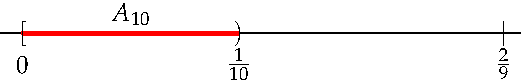
\includegraphics{setsii-06-intervalex}
	\end{minipage}
	\medbreak

	By modifying the endpoints of the sets $A_n$ we obtain slightly different results:
	\[
		\bigcap_{n=1}^\infty \bigl(0,\tfrac 1n) =\emptyset \qquad \bigcap_{n=1}^\infty \bigl(0,\tfrac 1n] =\emptyset\qquad \bigcap_{n=1}^\infty \bigl[0,\tfrac 1n] =\{0\}
	\]
	How would the arguments differ from what we did above?
\end{example}


\footnotetext{The existence of $N\ge\frac 1x$ should be intuitive; it is in fact guaranteed by the Archimedean property (Exercise \ref*{sec:proof2}.\ref{exs:archimedes}).}


The moral is that you cannot naïvely apply limits to sequences of sets. If thinking about limits helps your intuition, great, but you can't trust it blindly!\bigbreak

An indexed collection can also be nested the other way round, in which case the intersection is straightforward (though unions need more work)
\[
	A_1\subseteq A_2\subseteq A_3\subseteq\cdots \implies {\bigcap_{n=1}^\infty} A_n=A_1
\]
%though the union requires more work.

 
\begin{examples}{}{}
	Here are a few more simple examples of computing unions and intersections of indexed collections; some are nested, some not.
	\begin{enumerate}
		\item\label{ex:index2} Let $A_n=[n,n+1)\subseteq\R$, for each $n\in\Z$. For example $A_3=[3,4)$ and $A_{-17}=[-17,-16)$. Every real number lies in precisely one such set (the sets $A_n$ are pairwise disjoint), whence
		\[
			\bigcup\limits_{n\in\Z}A_n=\R\quad\text{and}\quad\bigcap\limits_{n\in\Z}A_n=\emptyset
		\]
		To prove the former, note that $x\in[n,n+1)$ where $n=\lfloor x\rfloor$ is the greatest integer less than or equal to $x$: i.e., $\forall x\in\R$, we have $x\in A_{\lfloor x\rfloor}$, whence $\R\subseteq\bigcup_{n\in\Z} A_n$ (the reversed subset inclusion is trivial since each $A_n\subseteq \R$).

		\item For each $n\in\N$, let $A_n=[-n,n]$ be a closed interval. This is a nested collection
		\[
			A_1\subseteq A_2\subseteq A_3\subseteq\cdots \implies {\bigcap_{n=1}^\infty} A_n=A_1=[-1,1]
		\]
		Similarly to the previous example, $\forall x\in\R$ we have $x\in A_n$ where $n$ is any integer $\ge\nm x$: we conclude that $\bigcup_{n=1}^\infty A_n=\R$. 

	
		\item For each $n\in\N$, let $A_n=\{x\in\R:\nm{x^2-1}<\frac 1n\}$. Before computing the union and intersection of these sets, it is helpful to write each set as a pair of intervals. Note that
	\[
		\nm{x^2-1}<\frac 1n\iff -\frac 1n< x^2-1<\frac 1n\iff \sqrt{1-\frac 1n}< \nm x< \sqrt{1+\frac 1n}
	\]
	\begin{minipage}[t]{0.6\linewidth}\vspace{0pt}
		The sets are nested: $A_1\supseteq A_2\supseteq A_3\supseteq A_4\supseteq\cdots$, where
		\begin{gather*}
			A_n=\left(-\sqrt{1+\tfrac 1n},-\sqrt{1-\tfrac 1n}\right)\cup\left(\sqrt{1-\tfrac 1n},\sqrt{1+\tfrac 1n}\right) \\
			\implies \bigcup_{n=1}^\infty A_n=A_1=(-\sqrt{2},0)\cup(0,\sqrt{2})
		\end{gather*}
		For the intersection,
	\end{minipage}
	\hfill
	\begin{minipage}[t]{0.39\linewidth}\vspace{0pt}
		\hfill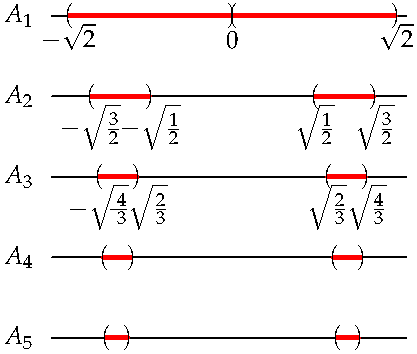
\includegraphics{setsii-05-intervalex}
	\end{minipage}
		\[
			\forall n\in\N,\ x\in A_n\iff \forall n\in\N,\ \nm{x^2-1}<\frac 1n \iff x^2-1=0
		\]
		It follows that $\bigcap_{n=1}^\infty A_n=\{1,-1\}$.
		
		\item Let $A_0=\{0,1\}$, $A_n=\{1\}$ is $n\ge 1$ is odd, and $A_n=\{2\}$ if $n\ge 2$ is even. Then,
		\[
			\bigcap_{n=1}^\infty\bigcup_{k=n}^\infty A_k = \left(\bigcup_{k=1}^\infty A_k\right)\cap\left(\bigcup_{k=2}^\infty A_k\right)\cap \cdots = \{0,1,2\}\cap\{0,1\}\cap\{0,1\}\cap\cdots =\{0,1\}
		\]
		Think about why $x\in \bigcap_{n=1}^\infty\bigcup_{k=n}^\infty A_k \Longleftrightarrow x$ lies in infinitely many of the sets $A_n$.
	\end{enumerate}
\end{examples}


\boldsubsubsection{Unions: Don't Confuse Sets and Elements}

When working with large unions, it is easy to confuse two sets:
\begin{itemize}\itemsep2pt
  \item $\{A_n\}$ is a set of sets, each element of which is some set $A_n$.
  \item $\bigcup A_n$ is the set whose elements lie in at least one $A_n$.
\end{itemize}
It is important to understand the difference! Sometimes the indexed collection itself is the object of interest, other times we may want to use its union or intersection to define something new.



\begin{example}[lower separated=false, sidebyside, sidebyside align=top seam, sidebyside gap=0pt, righthand width=0.3\linewidth]{Projective space}{projline}
	Let $A_m$ be the line\footnotemark{} through the origin in $\R^2$ with gradient $m\in\R\cup\{\infty\}$. 	Since every point in $\R^2$ lies on such a line, and distinct lines intersect at the origin, we see that
	\[
		\bigcup A_m=\R^2 \quad \text{and} \quad \bigcap A_m=\bigl\{(0,0)\bigr\}
	\]
  The indexed collection is known as \emph{projective space} 
  \tcblower
	\hfill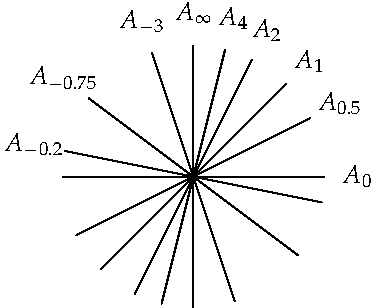
\includegraphics[scale=0.85]{setsii-03-projective}
\end{example}

\vspace*{-45pt}

\begin{tcolorbox}[exstyle]
	\[
  	\pr(\R^2)=\bigl\{A_m:m\in \R\cup\{\infty\}\bigr\}
  \]
	and is interesting in its own right. Each \emph{element} of projective space is a \emph{line}, making $\pr(\R^2)$ a very different set to $\R^2$. This example also shows that indexing sets don't have to be simple sets of integers! %It is also possible to index the same set using $I=[0,\pi)$. If we define $B_\theta$ to be the line through the origin making an angle $\theta$ with the positive $x$-axis, then $B_\theta=A_{\tan\theta}$.
\end{tcolorbox}

\footnotetext{The symbol $\infty$ is used to indicate the vertical line $A_\infty$ with `infinite gradient.'}

% 		\item For each $n\in\{1,2,3\}$, consider the \emph{plane} $A_n=\bigl\{(x,y,z):x+ny+n^2z=1\bigr\}\subseteq\R^3$.\par
% 		The indexed collection $\{A_1,A_2,A_3\}$ has \emph{three} elements: the planes $A_1,A_2,A_3$.\par
% 	  The union $A_1\cup A_2\cup A_3$ is an \emph{infinite} set: all points lying on \emph{at least one} of the three planes.\par
% 	  For the intersection, solve some simultaneous equations:
% 	  \[
% 	  	(x,y,z)\in\negthickspace\negthickspace\bigcap_{n\in\{1,2,3\}}\negthickspace\negthickspace A_n\iff
% 	  	\begin{cases}
% 	  		x+y+z=1\\
% 	  		x+2y+4z=1\\
% 	  		x+3y+9z=1
% 	  	\end{cases}
% 	  	\iff (x,y,z)=(1,0,0)
% 	  \]
% 	  Thus $\bigcap A_n=\bigl\{(1,0,0)\bigr\}$. The planes are drawn below.

	
% \begin{center}
% 	\begin{tabular}{c@{\qquad\qquad}c}
% 		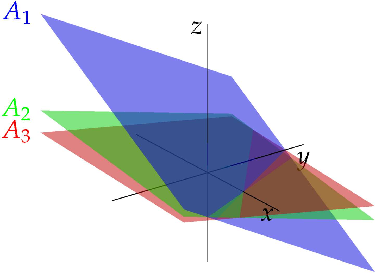
\includegraphics{setsii-01-planes}
% 		&
% 		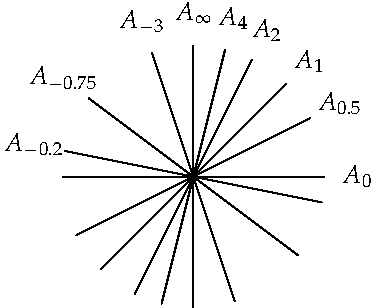
\includegraphics{setsii-03-projective}
% 		\\
% 		Three elements or infinitely many?
% 		&
% 		Projective space $\mathbb P(\R^2)$
% 	\end{tabular}
% \end{center}

%

In the next example we use an infinite union to define an interesting set.

\begin{example}{Finite Decimals}{finitedec}
	For each $n\in\N$, let $A_n$ be the set of decimals of length $n$,
	\[
		A_n=\bigl\{0.a_1a_2\ldots a_n:\text{where each $a_i\in\{0,1,\ldots,9\}$}\bigr\}
	\]
	For example $0.134\in A_3$. Since $0.134=0.1340$, we also have $0.134\in A_4$. This is a nested collection
	\[
		A_1\subseteq A_2\subseteq A_3\subseteq A_4\subseteq\cdots \implies \smash[b]{\bigcap_{n\in\N}}A_n=A_1=\bigl\{0,0.1,\ldots,0.9\bigr\}
	\]
	Now consider unions. If $m\in\N$, then
	\[
		\smash{\bigcup_{n=1}^m}A_n=A_m=\bigl\{x\in [0,1):x\text{ has a decimal representation of length $\le m$}\bigr\}
	\]
	You might guess that the infinite union would be the entire\footnotemark{} interval $[0,1]$, but this is incorrect:
	\begin{align*}
		x\in\bigcup_{n\in\N}A_n &\iff\exists n\in\N\text{ such that }x\in A_n\\
		&\iff x\text{ is a decimal with some \emph{finite} length $n$}
	\end{align*}
	The infinite union $\bigcup A_n$ is precisely the set of $x\in[0,1)$ which have a \emph{finite} decimal representation! This is far from the entire interval: many rational numbers are excluded (e.g., $\frac 13=0.3333\cdots \notin\bigcup A_n$), and the union contains \emph{no irrational numbers}. %in $\bigcup\limits_{n\in\N}A_n$:
% 	\[
% 		x\in A_n\implies y=10^nx\in\N \implies x=\frac y{10^n}\in\Q
% 	\]
%Many rational numbers are also excluded. For example .
\end{example}

\footnotetext{We would include $1=0.9999\cdots$}

\goodbreak


%\boldsubsubsection{Cantor's Middle-third Set}%\label{ex:cantor}

\boldinline{Optional!} We finish this section with a bit of fun, using an infinite intersection to create a \emph{fractal} set.

\begin{example}{Cantor's middle-third set}{cantorthird}
	Starting with the interval $C_0=[0,1]$, construct a sequence of sets $C_n$ by repeatedly removing the middle third of all intervals in $C_n$.\par
	
	\begin{minipage}[t]{0.45\linewidth}\vspace{-15pt}
		\begin{align*}
			C_0&=[0,1]\\
			C_1&=[0,\tfrac 13]\cup [\tfrac 23,1]\\
			C_2&=[0,\tfrac 19]\cup [\tfrac 29,\tfrac 13]\cup [\tfrac 23,\tfrac 79]\cup [\tfrac 89,1]\\
			&\mathrel{\,\,\vdots}
		\end{align*}
	\end{minipage}
	\hfill
	\begin{minipage}[t]{0.54\linewidth}\vspace{-10pt}
		\hfill \href{http://www.math.uci.edu/~ndonalds/math13/cantoranim.html}{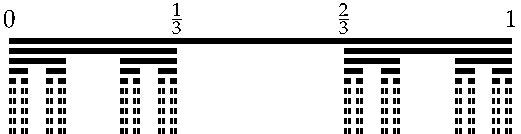
\includegraphics{setsii-02-cantor}}
	\end{minipage}
	\par

	The sequence is drawn up to $C_9$, though you'll have to zoom in a long way to see the detail!\par

	\emph{Cantor's middle-third set} is defined to be the infinite intersection $\mathcal C:=\negthickspace\bigcap\limits_{n=0}^\infty\negthickspace C_n$.\par

	Cantor's set has several interesting properties which we state non-rigorously.
	\begin{description}\itemsep2pt
		\item[Zero Measure (length)] It should seem reasonable to write
		\[
			\operatorname{len}(C_0)=1,\quad \operatorname{len}(C_1)=\tfrac 23,\quad\operatorname{len}(C_2)=\left(\tfrac 23\right)^2,\quad \ldots\quad ,\quad \operatorname{len}(C_n)=\left(\tfrac 23\right)^n,\quad\ldots
		\]
		where $\operatorname{len}(C_n)$ is the sum of the lengths of all intervals in $C_n$. Since $\mathcal C\subseteq C_n$ for all $n$, we conclude that $\operatorname{len}(\mathcal C)=0$: Cantor's set contains \emph{no intervals} of positive length.
	
		\item[Infinite Cardinality] Cantor's set contains the endpoints of every interval removed at any stage of its construction. In particular, $\frac 1{3^n}\in\mathcal C$ for all $n\in\N_0$, whence $\mathcal C$ is an \emph{infinite set}.\footnotemark
	
		\begin{minipage}[t]{0.6\linewidth}\vspace{-2pt}
		\item[Self-similarity] Let $f,g:\R\to\R$ be functions $f(x)=\frac 13 x$ and $g(x)=\frac 13x+\frac 23$. Since $C_{n+1}=f(C_n)\cup g(C_n)$, we conclude
		\[
			\mathcal C=\textcolor{red}{f(\mathcal C)}\cup \textcolor{blue}{g(\mathcal C)}
		\]
		\end{minipage}
		\hfill
		\begin{minipage}[t]{0.39\linewidth}\vspace{-4pt}
			\hfill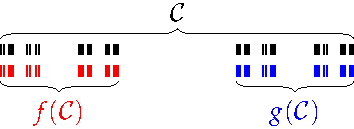
\includegraphics{setsii-09-cantorselfsim}
		\end{minipage}
		\smallbreak
		
		Cantor's set consists of \emph{two shrunken copies of itself}, a classic property of fractals.
	\end{description}

\end{example}

\footnotetext{In fact it is more than merely infinite, it is \emph{uncountably} so, as we'll discuss in Chapter \ref{chap:cantor}. The bizarre contrast between this and the zero measure property was part of the reason Cantor introduced his set.}

We'll analyze Cantor's set a little and consider a related construction in Exercises \ref{exs:cantorset} \& \ref{exs:modsnowflake}. Other fractal sets with a similar construction include the \emph{Sierpiński carpet} and the \emph{von Koch snowflake}.



\begin{exercises}{}{}
	A reading quiz and several questions with linked video solutions can be found \href{http://www.math.uci.edu/~ndonalds/math13/selftest/6-3-indexed.html}{online}.

	\begin{enumerate}
	  \item Let $I=\{1,3,4\}$. Determine $\bigcup_{r\in I}S_r$ and $\bigcap_{r\in I}S_r$, where each $S_r=[r-1,r+3]$ is an interval.
	  
	  
	  \item For each integer $n$, consider the set $B_n=\{n\}\times\R$.
		\begin{enumerate}
			\item Draw a picture (in the Cartesian plane) of $\bigcup_{n=2}^4B_n=B_2\cup B_3\cup B_4$.
			\item Draw a picture of the set $C=[1,5]\times\{-2,2\}$.\par
			(\emph{Careful! $[1,5]$ is an interval, while $\{-2,2\}$ is a set containing two points})
			\item Compute $\left(\bigcup_{n=2}^4B_n\right)\cap C$.
			\item Compute $\bigcup_{n=2}^4\left(B_n\cap C\right)$. Compare with your answer to part (c).
		\end{enumerate}
	  
	  
	  \goodbreak
	
	
	  \item Give an example of four subsets $A,B,C,D$ of $\{1,2,3,4\}$ such that all intersections of two subsets are different.
	
	
	  \item For each of collection, define an interval $A_n$ such that the given collection is $\{A_n:n\in\N\}$. Then find both the union and intersection of the collection.
	   \begin{enumerate}
	     \item $\bigl\{[1,2+1),\,[1,2+\frac 12),\,[1,2+\frac 13),\,\ldots\bigr\}$
	     \item $\bigl\{(-1,2),\,(-\frac 32,4),\,(-\frac 53,6),\,(-\frac 74,8),\,\ldots\bigr\}$
	     \item $\bigl\{(\frac 14,1),\,(\frac 18,\frac 12),\,(\frac 1{16},\frac 14),\,(\frac 1{32},\frac 18), \,(\frac 1{64},\frac 1{16}),\,\ldots\bigr\}$
	   \end{enumerate}
	  
	  
	%   \item For each non-negative real number $r\ge 0$ let 
	%   \[A_r=\big\{(x,y)\in\R^2:x^2+y^2=r^2\big\}\]
	% 		\begin{enumerate}
	%   		\item Describe each of the sets $A_r$ geometrically.
	%   		\item Prove that $\bigcup_{r\in\R^+_0}A_r=\R^2$.
	% 		\end{enumerate}
	
	
	  \item For each real number $x$, let $A_x=\{3,-2\}\cup\{y\in\R:y>x\}$. Find $\bigcup_{x\in\R}A_x$ and $\bigcap_{x\in\R}A_x$.
	  
	  
	  \item Use Definition \ref{defn:indexed} to prove that $A_1\subseteq A_2\subseteq A_3\subseteq\cdots\implies \bigcap_{n\in\N}A_n=A_1$
		
	
	%   \item Let $C_0(\R)$ denote the set of continuous functions $f:\R\to\R$ which satisfy $f(0)=0$.\\
	%   Let $A_f=\{x\in[0,1]:f(x)=0\}$ (so, for example, if $f:\R\to\R,\,x \mapsto x(2x-1)$, then $A_f=\{0,\frac 12\}$).
	%     \emph{Prove} that
	%   \[\bigcup\limits_{f\in C_0(\R)}\negthickspace\negthickspace A_f=[0,1]\qquad\text{and}\qquad\bigcap\limits_{f\in C_0(\R)}\negthickspace\negthickspace A_f=\{0\}.\]
			
			
		\item Let $A_n$ be the set of decimals of length $n$, as described in Example \ref{ex:finitedec}.
		\begin{enumerate}
		  \item Prove \emph{directly} that the cardinality of $A_n$ is $10^n$. 
		  \item Prove \emph{by induction} that $\nm{A_n}=10^n$.
		  \item Prove that $\bigcup_{n=1}^\infty A_n\subseteq\Q$.
			\item Explain why $\frac 19\notin\bigcup_{n=1}^\infty A_n$.
		\end{enumerate}
	
	
	  \item Suppose that $\forall n\in\N,\ A_n\neq\emptyset$ and $m\ge n\Longrightarrow A_m\subseteq A_n$. Prove or disprove the following:
	  \begin{enumerate}
	    \item $\bigcup\limits_{n=1}^{293}A_n\neq\emptyset$\qquad\quad 
	    (b) \ $\bigcap\limits_{n=1}^{293}A_n\neq\emptyset$\qquad\quad
	    (c) \ $\bigcup\limits_{n\in\N} A_n\neq\emptyset$\qquad\quad 
	    (d) \ $\bigcap\limits_{n\in\N} A_n\neq\emptyset$
		\end{enumerate}
		
		
		\item Compute the set $\bigcup_{n=1}^\infty\bigcap_{k=n}^\infty [\frac 1k,2+\frac 1k]$. For a general family of sets $\{A_n:n\in\N\}$ Explain why it is is reasonable to write
		\[
			x\in \bigcup_{n=1}^\infty\bigcap_{k=n}^\infty A_k\iff x\text{ lies in all except finitely many $A_n$}
		\]
		
		
		\item Let $\{A_n:n\in I\}$ and $\{B_n:n\in I\}$ be indexed families of sets. Give explicit examples for which the following hold:
		\begin{enumerate}
	    \item $\left(\bigcup_{n\in I} A_n\right) \cap \left(\bigcup_{n\in I}B_n\right) \neq \bigcup_{n\in I} (A_n \cap B_n)$
	    \item $\left(\bigcap_{n\in I} A_n\right) \cup \left(\bigcap_{n\in I}B_n\right) \neq \bigcap_{n\in I} (A_n \cup B_n)$
		\end{enumerate}
	
		
		\item (De Morgan's laws)\lstsp Let $\{A_n:n\in I\}$ be an indexed family of sets and $B$ a set. Prove
		\begin{enumerate}
	    \item $B\setminus \left(\bigcup_{n\in I} A_n\right) = \bigcap_{n\in I} (B\setminus A_n)$
	    \item $B\setminus \left(\bigcap_{n\in I} A_n\right) = \bigcup_{n\in I}(B\setminus A_n)$
		\end{enumerate}
		
		
		\item Suppose we are working in a universal set $\cU$ (so every set is considered a subset of $\cU$). Give an explanation for why it makes sense to define $\bigcap_{n \in I} A_n = \cU$ when $I = \emptyset$.
		
		\goodbreak
		
		\item (Hard) Let $A_n=\{\frac mn\in\Q:0<m<n, m\in \N\}$, for each $n\in\N$.
		\begin{enumerate}\itemsep1pt
			\item State $A_1,A_2,A_3,A_4$ explicitly.
			\item Prove that $A_m\subseteq A_{pm}$ for any $p\in\N$.
			\item Argue that $\bigcup_{n\in\N}A_n=\Q\cap (0,1)$.
			\item Argue that further $\bigcup_{n\in\N}A_{2n}=\Q\cap (0,1)$.
			\item Extend your proof to show that, for any fixed $p\in\N$, $\bigcup_{n\in\N}A_{pn}=\Q\cap (0,1)$.
		\end{enumerate}
		
		\goodbreak
		
			
		\item\label{exs:cantorset} (Hard)\lstsp A \emph{ternary representation}\footnotemark{} of a number $x\in[0,1]$ is an expression
		\[
			x=\sum\limits_{n=1}^\infty \frac{a_n}{3^n}=\frac{a_1}{3}+\frac{a_2}{3^2}+\frac{a_3}{3^3}+\cdots \text{ where each }a_n\in\{0,1,2\}
		\]
		We write $x=[0.a_1a_2a_3\cdots]_3$. For example $[0.12]_3=\frac 13+\frac 2{3^2}=\frac 59$.
		\begin{enumerate}
		  \item Verify that $[0.02101]_3=\frac{64}{243}$, \ $[0.22222\cdots]_3=1$ and $[0.020202020\cdots]_3=\frac 14$.\par
		  (\emph{Hint: You'll need the geometric series formula $\sum_{n=1}^\infty r^n=\frac r{1-r}$ for the latter two})
		  
		  \item Let $C_n$ be the $n\th$ set in the construction of Cantor's middle-third set $\mathcal C$ (Example \ref{ex:cantorthird}).\par
		  Prove by induction that $C_n$ is the set of all $x\in[0,1]$ with a ternary representation whose first $n$ digits are only 0 or 2.\par
		  (\emph{Hints: Use $C_{n+1}=f(C_n)\cup g(C_n)$; What does division by 3 do to a ternary representation?})
		  	  
		  \item Argue that $\frac 14\in\mathcal C$, but that it is not an endpoint of any of the deleted middle-thirds removed during the construction of $\mathcal C$.
		\end{enumerate}
		
		
		\item\label{exs:modsnowflake} (Hard)\lstsp We construct a modified Cantor set and fractal curve. Starting with $F_0=[0,1]$, repeatedly delete the \emph{third quarter} segment of each interval to obtain a sequence of sets $F_0,F_1,F_2,\ldots$:
	  \begin{gather*}  
	  	F_1=[0,\tfrac 12]\cup[\tfrac 34,1],\quad
	  	F_2=[0,\tfrac 14]\cup[\tfrac 38,\tfrac 12]\cup[\tfrac 34,\tfrac 78]\cup[\tfrac{15}{16},1],\quad \ldots
	  \end{gather*}
	  \begin{enumerate}
	    \item Prove that the sum of the lengths of all of all line segments in $F_n$ is $\left(\frac 34\right)^n$.
	    \item Prove that $\bigcap_{n=1}^\infty F_n$ contains no intervals of positive length.
	    
	    \begin{minipage}[t]{0.62\linewidth}\vspace{-5pt}
	    \item Instead of deleting the third quarter of each line segment, replace it with the other three sides of a square. The first three steps and the result of applying the process infinitely many times are shown in the pictures.\smallbreak
	
	    After step 1 the curve has length $\ell_1=\frac 32$ and the area under the curve is $A_1=\frac 1{4^2}$. After step 2 the length is $\ell_2=\frac 94$ and the area $A_2=A_1+\frac 14A_1+\frac 1{16}A_1 =\frac{21}{4^4}$. 
	    \begin{enumerate}\itemsep0pt
	      \item Find the length $\ell_n$ of the curve after $n$ steps. What is the `length' of the resulting fractal curve?
	      \item Repeat for the \emph{area} under each curve $F_n$. Prove that the area between the fractal and the $x$-axis is $\frac 18$.
	    \end{enumerate}
	    \end{minipage}
	    \hfill
	    \begin{minipage}[t]{0.35\linewidth}\vspace{-25pt}
	    \flushright
	    	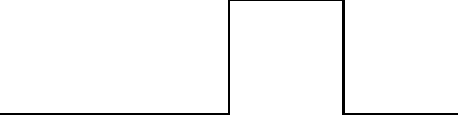
\includegraphics[scale=0.64]{fractal1}
	    	\\
	    	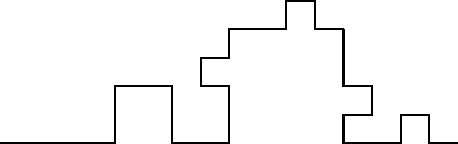
\includegraphics[scale=0.64]{fractal2}
	    	\\
	    	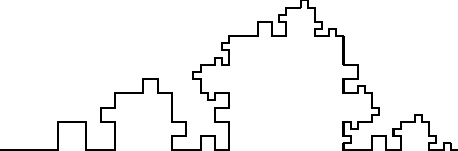
\includegraphics[scale=0.64]{fractal3}
	    	\\
	    	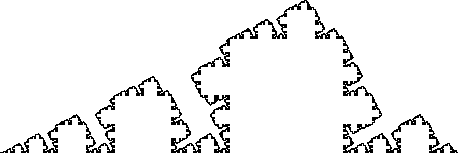
\includegraphics[scale=0.64]{fractal}
	    \end{minipage}
		\end{enumerate}


% 
% \item Let $\{A_n : n \in I\}$ be an indexed family of sets and $B$ a set. Prove
% \begin{enumerate}
%     \item \[\left(\bigcup_{n \in I} A_n \right) \setminus B = \bigcup_{n \in I} (A_n \setminus B)\]
%     \item \[\left(\bigcap_{n \in I} A_n \right) \setminus B = \bigcap_{n \in I} (A_n \setminus B)\]
% \end{enumerate}

% \item We can take the Cartesian product of arbitrarily many sets. Let $\{A_n : n \in I\}$ be a family of sets. Define
% \[
% \prod_{n \in I} A_n = \left\{f : I \to \bigcup_{n \in I} A_n \bigm| f(n) \in A_n\right\}.
% \]
% \begin{enumerate}
%     \item If $I = \N$ and $A_n = \R$ for each $n \in \N$, can you give a more intuitive description of the elements of $\prod_{n \in \N} A_n$?
%     \item Suppose we have two families $\{A_n : n \in I\}$ and $\{B_n : n \in I\}$. Prove
%     \[
%         \left(\prod_{n \in I} A_n \right) \cap \left(\prod_{n \in I} B_n \right) = \prod_{n \in I} (A_n \cap B_n)
%     \]
% \end{enumerate}

% 	\item Let $X$ be a set. A collection of sets $\tau \subseteq \cP(X)$ is called a \emph{topology} if the following conditions are satisfied:
% \begin{enumerate}
%     \item $\emptyset \in \tau$ and $X \in \tau$;
%     \item $\tau$ is closed under arbitrary union. That is, if $\{U_n : n \in I\} \subseteq \tau$ for any index set $I$, then $\bigcup_{n \in I} U_n \in \tau$;
%     \item $\tau$ is closed under finite intersection. That is, if $U_1,\ldots,U_n \in \tau$ for any $n \in \N$, then $U_1 \cap \cdots \cap U_n \in \tau$.
% \end{enumerate}
% Elements of $\tau$ are called \emph{open sets}.
% \begin{enumerate}
%     \item Let $X = \{a,b,c,d\}$. Let $\tau_1 = \{\emptyset, X\}$, $\tau_2 = \cP(X)$, $\tau_3 = \{\emptyset, \{d\}, \{a,b\}, \{b,c\}, \{a,b,c\}, X\}$, and $\tau_4 = \{\emptyset, \{b\}, \{a,b\}, \{b,c\}, \{a,b,c\}, X\}$. Show $\tau_1,\tau_2$ and $\tau_4$ are topologies while $\tau_3$ is not.
%     
%     \item Let $X$ be an infinite set and define $\tau = \{A \in \cP(X) : X \setminus A \text{ is finite}\} \cup \{\emptyset\}$. Show $\tau$ is a topology.
%     \item The \emph{standard topology} $\tau$ on $\R$ can be defined by declaring that a set $U \subseteq \R$ is open (i.e. an element of $\tau$) if and only if for every $x \in U$, there is an open interval $(a,b)$ such that $x \in (a,b)$ and $(a,b) \subseteq U$. Show this defines a topology on $\R$.
% \end{enumerate}
% 
% \item Let $X$ be a set and $\tau$ a topology on $X$. A set $C \subseteq X$ is called \emph{closed} if its complement is open, i.e., if $X \setminus C \in \tau$. 
% \begin{enumerate}
%     \item Show the following properties of closed sets:
%     \begin{enumerate}
%         \item $\emptyset$ and $X$ are both closed.
%         \item If $\{A_n : n \in I\}$ is an arbitrary collection of closed sets, then $\bigcap_{n \in I} A_n$ is closed.
%         \item If $A_1,\ldots,A_n$ are closed sets, then $A_1 \cup \cdots \cup A_n$ is closed.
%     \end{enumerate}
%     \item In the standard topology on $\R$, show that a closed interval $[a,b]$ is a closed set but that a half-open interval $[a,b)$ is neither open nor closed.
% \end{enumerate}
	\end{enumerate}

\end{exercises}
	
	
	\vspace{-20pt}
	


\footnotetext{Analogous to a decimal representation $x=\sum_{n=1}^\infty \frac{a_n}{10^n}=\frac{a_1}{10}+\frac{a_2}{10^2}+\frac{a_3}{10^3}+\cdots$ where $a_n\in\{0,1,2,\ldots,9\}$.}

